%; whizzy chapter
% -initex iniptex -latex platex -format platex -bibtex jbibtex -fmt fmt
% 以上 whizzytex を使用する場合の設定。

%     Kansai Debian Meeting resources
%     Copyright (C) 2007 Takaya Yamashita
%     Thank you for Tokyo Debian Meeting resources

%     This program is free software; you can redistribute it and/or modify
%     it under the terms of the GNU General Public License as published by
%     the Free Software Foundation; either version 2 of the License, or
%     (at your option) any later version.

%     This program is distributed in the hope that it will be useful,
%     but WITHOUT ANY WARRANTY; without even the implied warranty of
%     MERCHANTABILITY or FITNESS FOR A PARTICULAR PURPOSE.  See the
%     GNU General Public License for more details.

%     You should have received a copy of the GNU General Public License
%     along with this program; if not, write to the Free Software
%     Foundation, Inc., 51 Franklin St, Fifth Floor, Boston, MA  02110-1301 USA

%  preview (shell-command (concat "evince " (replace-regexp-in-string "tex$" "pdf"(buffer-file-name)) "&"))
% 画像ファイルを処理するためにはebbを利用してboundingboxを作成。
%(shell-command "cd image200708; ebb *.png")

%%ここからヘッダ開始。

\documentclass[mingoth,a4paper]{jsarticle}
\usepackage{kansaimonthlyreport}
\usepackage[dvips]{xy}
\usepackage{ulem}

% 日付を定義する、毎月変わります。
\newcommand{\debmtgyear}{2013}
\newcommand{\debmtgdate}{26}
\newcommand{\debmtgmonth}{5}
\newcommand{\debmtgnumber}{72}

\begin{document}

\begin{titlepage}

% 毎月変更する部分、本文の末尾も修正することをわすれずに

 第\debmtgnumber{}回 関西 Debian 勉強会資料

\vspace{2cm}

\begin{center}
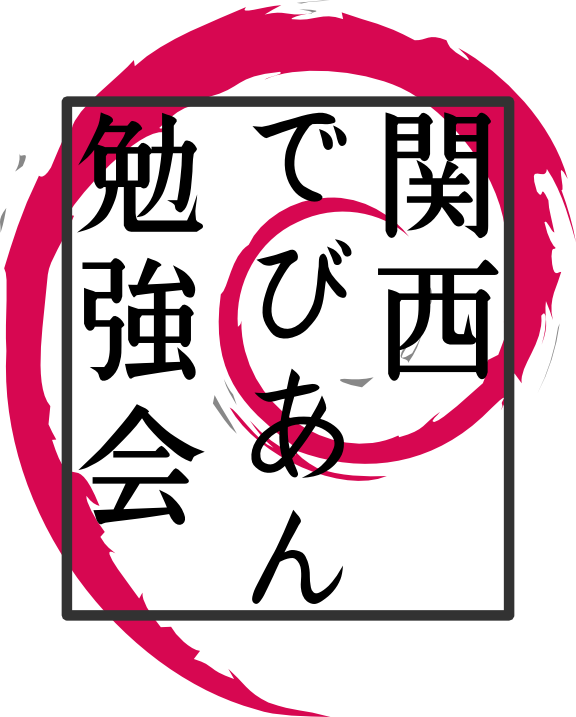
\includegraphics{image200802/kansaidebianlogo.png}
\end{center}

\begin{flushright}
\hfill{}関西 Debian 勉強会担当者 佐々木・倉敷・のがた・かわだ・八津尾 \\
\hfill{}\debmtgyear{}年\debmtgmonth{}月\debmtgdate{}日
\end{flushright}

\thispagestyle{empty}
\end{titlepage}

\dancersection{Introduction}{Debian JP}

\vspace{1em}

 関西Debian勉強会はDebian GNU/Linuxのさまざまなトピック
 (新しいパッケージ、Debian特有の機能の仕組、Debian界隈で起こった出来事、
 などなど)について話し合う会です。

 目的として次の三つを考えています。
 \begin{itemize}
  \item MLや掲示板ではなく、直接顔を合わせる事での情報交換の促進
  \item 定期的に集まれる場所
  \item 資料の作成
 \end{itemize}

 それでは、楽しい一時をお楽しみ下さい。

\newpage

\begin{minipage}[b]{0.2\hsize}
 {\rotatebox{90}{\fontsize{80}{80}
{\gt 関西 Debian 勉強会}}}
\end{minipage}
\begin{minipage}[b]{0.8\hsize}
\hrule
\vspace{2mm}
\hrule
\setcounter{tocdepth}{1}
\tableofcontents
\vspace{2mm}
\hrule
\end{minipage}

\dancersection{最近のDebian関係のイベント報告}{Debian JP}

\subsection{第 71 回関西 Debian 勉強会}

71 回目の関西 Debian 勉強会は 4 月 28 日(日)に福島区民センターで行な
われました。

倉敷さんの「クラウド初心者が AWS に Debian をのっけて翻訳サービスの試
行に挑戦してみた」と佐々木さんの「リリースノートを読んでみよう。」の二
本でした。

参加者でクラウドを使ったことがある人は以外と少かったです。
紹介されたクラウド上で動いているサービス DebianJP Web Translation
\footnote{\url{http://lurdan.dip.jp/}} も活用して Debian の翻訳
をよくしていけるよう反応をいただけるとありがちですね。

リリースノートは読んでたつもりでしたが、人が読まれた内容を聞いていると
見落しているなと思うところがあって、いろんなことに気づかされた内容でし
た。


\subsection{第 100 回東京エリア Debian 勉強会}
ついに 100 回となった第 100 回東京エリア Debian 勉強会は 5 月 11 日
(土) に渋谷ファーストプレイスで開催されました。

いつもの勉強会とは趣きを変えてアンカンファレンス形式での開催となった今
回、どんな風に開催されたのかは参加レポート
\footnote{\url{http://henrich-on-debian.blogspot.jp/2013/05/100th-tokyo-debian-meeting-wheezy.html}}
か、Twitter ハッシュタグ \#tokyodebian100 を参照してみてください。


\subsection{Debian Project}

とうとう、ついに、ようやく、5 月 4 日に Debian 7.0 「Wheezy」 がリリース
\footnote{\url{http://www.debian.org/News/2013/20130504}}
されました。
みなさんもうインストール、そしてパーティはされましたか。

さっそくですが、Wheezy のポイントリリースが来月の 15 日に予定されてい
ます。
\footnote{\url{http://lists.debian.org/debian-release/2013/05/msg00524.html}}
なぜか 7.0.1 ではなく 7.1 となるようですが、こちらもチェックしておいて
ください。

そして、Wheezy がリリースされたということで、Jessie の開発が始まってい
ます。
\footnote{\url{http://lists.debian.org/debian-devel-announce/2013/05/msg00004.html}}
toolchain
\footnote{\url{http://lists.debian.org/debian-devel-announce/2013/05/msg00005.html}}
からさまざまなソフトウェアまで、連日 unstable のパッケージが更新されて
います。しばらく unstable から目が離せないでしょう。


\dancersection{事前課題}{Debian JP}

今回は以下の課題を出題しました.
\begin{screen}
  \begin{enumerate}
  \item %
    DebianとUbuntuの違いを挙げてみてください
  \item %
    Debianを使っていて/使い始めて/使おうとして、困った/ていることを、
    1件以上書いてください
  \end{enumerate}
\end{screen}
参加者の皆さんの解答は以下の通りです:

\begin{prework}{ 榎真治 }
  \begin{enumerate}
  \item 自由なオペレーティングシステムをめざすDebianと自由を重視しつつユーザーの利便性も重視しているUbuntuというミッションの違いがあるという理解です。

    また、完全なコミュニティベースのDebianとCanonicalがコミュニティの中で特別な地位をしめるUbuntuというプロジェクト体制の違いもあると思います。

    そのほかにも、リリースポリシーなども違います。

  \item メール環境WindowsのBeckyからSylpheedへ移行する際に、フォルダ単位でしかインポートできず、メールの数が多いとインポートがエラーになることがあり、手こずっています。

    スケジュールソフトで、サイボウズLiveと同期できるような方法がないかを探しています。
  \end{enumerate}
\end{prework}

\begin{prework}{ 山城の国の住人 久保博 }
  \begin{enumerate}
  \item
    \begin{itemize}
    \item 開発元の団体が違う
    \item リリースサイクルやサポートのライフサイクルが違う
    \end{itemize}
  \item 
    \begin{itemize}
    \item Debian wheezy のマシン二台で、マイクの音声が拾えなくて困っています。
    \item デスクトップ PC で grub (GRUB2) で Windows XP と Debian wheezy との dual boot にしていたのですが、いつの間にか Windows XP が起動しなくなりました。
    \item  GNOME3 に戸惑っています。まだ慣れません。
    \end{itemize}
  \end{enumerate}
\end{prework}

\begin{prework}{ Takubo.Morio }
  \begin{enumerate}
  \item 
    \begin{itemize}
    \item Debianの開発はコミュニティ。
    \item Ubuntuの開発は企業(Canonical)主体。
    \end{itemize}
  \end{enumerate}
\end{prework}

\begin{prework}{ スペンス }
  今のところDebianは普段使っていないけど、検討したいと思って、勉強会に参加させていただきたいです。
\end{prework}

\begin{prework}{ おくの }
  \begin{enumerate}
  \item デフォルトのデスクトップ環境が違う

    個人的にはUbuntuのUnityは割と好きです。

  \item GNOME3にまだ慣れていないので慣れるまで大変です。
  \end{enumerate}
\end{prework}

\begin{prework}{ murase\_{}syuka }
  \begin{enumerate}
  \item 
    \begin{itemize}
    \item gnome3 / unity
    \item stable / tested(unstable)
    \end{itemize}
  \item 
    \begin{itemize}
    \item VBox上のdebian64bitからdebian32bit環境への引越しする場合

      パッケージ構成が同じなら

      /etc, /home/user以下をcopyで問題なし?
    \item debianで使いやすい無料dnsサービスって?

      DynDNSが有料化されたので
    \item GNU/kfreebsdは運用可能なほど安定している?

      squeezeのときはインストールが成功しなかったので
    \item nVidia配布ドライバの行儀の良いインストール方法

      kernelの更新のたび?ドライバの再インストールしてたので
    \end{itemize}
  \end{enumerate}
\end{prework}

\begin{prework}{ 末廣 雅利 }
  \begin{enumerate}
  \item Ubuntu を使ったことないのでよく分かってないのですが、
    \begin{itemize}
    \item リリースサイクルが違う
    \item Ubuntu の方が導入の敷居が低く、使いやすい(イメージがある)
    \end{itemize}
  \item 
    \begin{itemize}
    \item Ruby のライブラリ

      Ruby のライブラリを Debian パッケージで入れるのか、自力で入れるのかで困ったことがありました。

      今は、rbenv + Bundler で済ませてしまっています。
    \item USBメモリからのインストールに挫折

      etch か lenny の頃、USBメモリからインストールしようと四苦八苦したが成功せず、
      結局、最小の CD を焼いてネットワークインストールしたことがあります。
    \end{itemize}
  \end{enumerate}
\end{prework}

\begin{prework}{ Sachy }
  \begin{enumerate}
  \item リリースの頻度が違う。開発している団体が違う。
  \item Debian Ubuntu共通のことですが、古いパッケージが欲しい時に手に入れられないことが多い。
  \end{enumerate}
\end{prework}

\clearpage

\begin{prework}{ kozo2 }
  \begin{enumerate}
  \item 同じpackage名でもbinaryが違う,必ずしも互換性があるわけではない
  \item netinst.isoで有線アダプタが無いマシンで無線ネットワークの検出に失敗した

    netinst.isoでうまくbootできなかった
  \end{enumerate}
\end{prework}

\begin{prework}{ 西山和広 }
  \begin{enumerate}
  \item Debian はユニバーサルオペレーティングシステムだけど Ubuntu は Linux のみで対応アーキテクチャも限定されている。

    Debian はすべての公式パッケージがセキュリティアップデートなどのサポート対象だが、Ubuntu は universe などサポート対象外のパッケージが多い。

    Debian はリリースが不定期だが、Ubuntu は定期的にリリースされている。
  \item zabbix が wheezy に入らなかった。
  \end{enumerate}
\end{prework}

\begin{prework}{ lurdan }
  \begin{enumerate}
  \item
    \begin{itemize}
    \item 独裁者 (と所有企業) の有無
    \item リリースサイクル
    \item 用途毎にバリエーションを作って使い捨てるか、単一の配布で多くの用途をカバーしようとするか、の方針
    \end{itemize}
  \item 表面化してないけど結構古いままのパッケージが最近目につくかも?
  \end{enumerate}
\end{prework}

\begin{prework}{ かわだてつたろう }
  \begin{enumerate}
  \item
    \begin{itemize}
    \item Debian の main と Ubuntu の main。
    \item DFSG と Ubuntu のライセンス。
    \item PPA の有無。
    \end{itemize}
  \item Debian だけではないですが、ディストリビューションとどのように付き合っていくか。

    最新バージョンがパッケージに無い場合やソフトウェア個別のパッケージ管理システムと相性がよくない場合など。
  \end{enumerate}
\end{prework}

\begin{prework}{ 川江 }
  \begin{enumerate}
  \item Debianはユーザーインターフェイスがシンプル。Ubuntuはユーザーインターフェイスが凝ってる( Unity etc.)
  \item 最新のハードや、希少のハードに対応してない事、また、Debian で走らすための「情報」が乏しい。
  \end{enumerate}
\end{prework}

\begin{prework}{ kyoko.oh }

(無回答)

\end{prework}

\begin{prework}{ kino }
  \begin{enumerate}
  \item
    \begin{itemize}
    \item Debianはコミュニティベース、UbuntuはCanonical社主導
    \item サポートポリシー。

      Debianは全パッケージサポート、UbuntuはmultiverseやuniverseはUbuntuチームとしてサポートされない。

    \item リリースサイクル

      Debian: メジャーバージョン1世代+1年間

      Ubuntu: 6か月サイクル 9か月間サポート+LTS 5年サポート

    \item 個別のパッケージの設定も微妙に違う。
    \end{itemize}
  \item
    \begin{itemize}
    \item 日本語で質問できるサイトってどこかにありますか?
    \item Ubuntuでの情報を流用しやすくするために、どこを読み替えればよいかがわかるとうれしい。
    \item アップグレードできる利点と引き換えに、サポート期間が短いのが結構つらい。2世代サポートが欲しいです。
    \item アップグレード時に意図して使っていないが依存で入ってくるパッケージのconfファイルを更新するかと聞かれてどう対処するか迷う時があります。

      アップグレード時のベストプラクティスを知りたいです。
    \item APT-Pinning 機能は素晴らしいのですが、理解が難しいのでハンズオンを希望します。
    \item 2chWikiの信頼出来る部分をdebian.or.jpの見やすい所に置けないでしょうか。
    \item Webアプリ系だとパッケージインストールすると逆にメンテナンスが難しくなることがあるので、素人アイデアとして、ファイルの分割をせずアップストリームtarの解凍そのままをパッケージに出来ないものでしょうか。
    \end{itemize}
  \end{enumerate}
\end{prework}

\begin{prework}{ 佐々木洋平 }

(無回答)

\end{prework}

\clearpage
\dancersection{%
  Debian と Ubuntu の違いを知ろう}{%
  西田}

\subsection{この話の趣旨}

「Linuxはとりあえず人気のあるUbuntuを使っている」という方は多いのでは
無いでしょうか。

この話はDebianとUbuntuの違いを挙げ、どちらがみなさんに適しているか考え
てみていただくことを目的としています。
また違いを知るのはお互い(ユーザーと開発者)の文化の違いの理解や相互の情
報交換によるDebian packageの質の向上にもつながるかと思います。

\subsection{supportされるarchitecture}

packageなどの違いについて考える前に、まず使おうとされているhardwareが
supportされていないとどうしようもありません。

Ubuntu(Raring Ringtail)ではIntel x86, AMD64(Macに特化したものもあ
り),OMAP(ARM)をsupportしています。Debianではこれらに加え、ARM複数種、
MIPS、powerpc、sparc、その他(その他のarchitectureについては無知であ
るため名称略)をsupportしています。

大部分の方はx86, amd64でDebian, Ubuntuを使うかとは思うのですが念のため。

\subsection{packageについて}

みなさんが最も気になるのは(PC用の)packageがどう異なるのか、ではないで
しょうか。ご存知のようにUbuntuのpackageはDebianをベースとしたものです。
ですが意外とそのpackageが

\begin{itemize}
\itemsep1pt\parskip0pt\parsep0pt
\item
  必ずしもbinary互換性があるわけでは無いこと
\item
  UbuntuのpackageはDebianのpackageをベースにUbuntu環境で
  \texttt{recompile}したものがほとんどであること
\item
  Debian由来のpackageのソースが具体的にどのように異なっているのか、ど
  うするとその違いが確認できるのか
\item
  Linux kernelはどのように異なっているか
\end{itemize}

といった所までご存知で、用いているDebian packageの違いをいつも確認され
ている方は少ないのではないでしょうか。

下記では上記の点に関して説明します。

\subsubsection{なぜUbuntuではDebian packageをrecompileしているのか}

まずUbuntu自体はUbuntuにdefaultのツールチェーン(gcc,
libcなどといったbuild
に欠かせないGNUのlibraryの集まりを意図しています)で完全にbuildできるようになっ
ているのですが、この要であるgccに元となるDebianと同じversionのものを用いる考
えがありません。
Ubuntuでは``新しいversionのgccはよりよいbinaryを作るはず''という考えのもと
出来る限り新しいgccを使おうとしているようです。そしてそのgccはまずDebian
より新しいversionのものとなるようです。
(たとえばUbuntu-Raringのgccは4.7.3、Debian-wheezyのgccは4.7.2です)

つまりDebianからsourceをもってきているのですがbuild環境を合わせる考え
はありません。そのためUbuntuとDebian間でpackageにbinary互換性は保証さ
れていません。こういったことからUbuntuはすべてのDebian packageを新しい
versionのツールチェーンでbuildしなおしています。

これはUbuntuのpackage repository区分で言うところの``Main''だけの話では無
く``universe''(communityによってsupportされているpackageの分類)について
も同様で、たとえばUbuntuの``Main''に含まれるPythonのversionが元となる
DebianのPythonより新しい場合、``universe''に含まれるPython packageも新し
いversionのPythonとの整合性を確保するためにrebuildされます。

\subsubsection{UbuntuとDebianで異なっているpackageの確認方法}

前項のように互換性を確保しrebuildできれば、Ubuntuでも元となるDebianと
同じversionのpackageができ問題は無いのですが、まれにそうはいかないもの
もあるのか、それ以外の事情があるのかUbuntu側でpackageの修正を行う必要
があるものが出てきます。

こういったpackageは
\url{https://launchpad.net/ubuntu/raring/+localpackagediffs?field.package_type=all}
で確認できます。ここではRaringとそのpackageの元となるWheezyのpackageの間で違いのあるも
のが列挙されており、それらを下記の3区分でfilterすることが可能になって
います。

\begin{itemize}
\itemsep1pt\parskip0pt\parsep0pt
\item
  無視できない違いがあったもの(古いversionを用いる、ubuntuなりの変更を入れ
  る必要があったもの)
\item
  Wheezyより新しいversionでなら上記のような問題は無かったもの
\item
  Wheezyと同じversionで問題無かったもの
\end{itemize}

現在(2013年5月26日)では 計17261件のうちそれぞれ

\begin{itemize}
\itemsep1pt\parskip0pt\parsep0pt
\item
  154件
\item
  5908件
\item
  11080件
\end{itemize}

となっています。

Ubuntu側の``ツールチェーンにできるだけ新しいものを使う''という方針が影響
しているのか``Wheezyより新しいversionでなら上記のような問題は無かったも
の''が多いようです。

\subsubsection{debdiffコマンドを用いたUbuntu, Debian packageの比較}

debdiffコマンドを用いると2package間の情報の比較ができます。
debdiffコマンドはdevscripts packageをinstallすることで使えるようになり
ます。 比較したい2packageのdsc, orig.tar.gz, debian.tar.gz, fileを適当な
directoryにdownload後、下記のようにdebdiffします。

\begin{commandline}
kozo2@ubuntu:~/tmp$ sudo aptitude -y install devscripts
kozo2@ubuntu:~/tmp$ ls
aptitude_0.6.8.1-2ubuntu2.debian.tar.gz  aptitude_0.6.8.1.orig.tar.xz      aptitude_0.6.8.2-1.dsc
aptitude_0.6.8.1-2ubuntu2.dsc            aptitude_0.6.8.2-1.debian.tar.gz  aptitude_0.6.8.2.orig.tar.xz
kozo2@ubuntu:~/tmp$ debdiff aptitude_0.6.8.2-1.dsc aptitude_0.6.8.1-2ubuntu2.dsc
gpgv: Signature made Wed 07 Nov 2012 02:54:14 PM JST using RSA key ID 4D6E25A8
gpgv: Can't check signature: public key not found
dpkg-source: warning: failed to verify signature on /home/kozo2/tmp/aptitude_0.6.8.2-1.dsc
gpgv: Signature made Tue 26 Feb 2013 05:28:12 PM JST using DSA key ID 0F932C9C
gpgv: Can't check signature: public key not found
dpkg-source: warning: failed to verify signature on /home/kozo2/tmp/aptitude_0.6.8.1-2ubuntu2.dsc

中略

--- aptitude-0.6.8.2/src/generic/apt/pkg_changelog.cc   2012-11-05 00:24:56.000000000 +0900
+++ aptitude-0.6.8.1/src/generic/apt/pkg_changelog.cc   2012-08-04 18:33:38.000000000 +0900
@@ -20,7 +20,6 @@
#include "pkg_changelog.h"

#include "apt.h"
-#include "config_signal.h"
#include "download_queue.h"

#include <generic/util/job_queue_thread.h>
@@ -543,18 +542,12 @@
else
realver = source_version;

-              // WATCH: apt/cmdline/apt-get.cc(DownloadChangelog)
-              string server = aptcfg->Find("APT::Changelogs::Server",
-                                           "http://packages.debian.org/changelogs");
-         string path = cw::util::ssprintf("pool/%s/%s/%s/%s_%s",
+         string uri = cw::util::ssprintf("http://packages.debian.org/changelogs/pool/%s/%s/%s/%s_%s/changelog",
realsection.c_str(),
prefix.c_str(),
source_package.c_str(),
source_package.c_str(),
realver.c_str());
-              string uri = cw::util::ssprintf("%s/%s/changelog",
-                                              server.c_str(),
-                                              path.c_str());
LOG_TRACE(logger,
"Adding " << uri
<< " as a URI for the changelog of " << source_package << " " << source_version);
diff -Nru aptitude-0.6.8.2/src/generic/apt/tasks.cc aptitude-0.6.8.1/src/generic/apt/tasks.cc
--- aptitude-0.6.8.2/src/generic/apt/tasks.cc   2012-11-05 00:24:56.000000000 +0900
+++ aptitude-0.6.8.1/src/generic/apt/tasks.cc   2012-08-25 21:39:57.000000000 +0900
@@ -80,7 +80,7 @@
++it)
{
pkgCache::PkgIterator pkg = (*apt_cache_file)->FindPkg(*it, arch);
-      if(pkg.end() == false)
+      if(pkg.end() != false)
pkgset->insert(pkg);
}

kozo2@ubuntu:~/tmp$
\end{commandline}

\subsubsection{Linux kernelの差異}

kernelもpackageなので触れないわけにはいかないですが、私はkernel hacker
ではなく語れる力はありません。申し訳ありません。configの違いを調べるこ
とは可能かと思います。Ubuntuのconfigは下記で参照可能ですが、Debianの
kernel configはどこで参照できるのか調べがつきませんでした。

\begin{itemize}
\itemsep1pt\parskip0pt\parsep0pt
\item
  \url{https://wiki.ubuntu.com/Kernel/Configs/QuantalToRaring}
\item
  \url{http://kernel.ubuntu.com/~kernel-ppa/configs/}
\end{itemize}

また、おそらく適用しているであろうUbuntu, Debian毎のpatchの差異までは
調べがつきませんでした。

\subsection{policyなどの違い}

次にpackageの内容のような具体的なことからすこし離れ、UbuntuとDebianの方針の
違いについてお話しします。このあたりはご存知の方も多いかと思うのですが
前節のpackageの新旧とも関わるので補足する意味で付記します。

\subsubsection{release policy}

Debianはstableのrelease時期が決まっていないのに対し、Ubuntuは定期的な新version
のreleaseが宣言されており、support期間も明確に決まっています。(とはいう
ものの本勉強会参加者はunstableのDebianを利用しており、かつ自己で問題を
解決する方が多いと思うので、一応書いた程度のものです)

\subsubsection{communityの違い、交流}

Ubuntuのcommunityにはマーク・シャトルワース氏のCanonical社との雇用関係
にある開発者が存在しており、この雇用関係が前述の定期releaseの実現、ま
た前節のpackageのbug修正に効いているようです。 (ただし世界各地のUbuntu
communityに関してはこの限りではありません)

こういったユーザー指向のUbuntuに対しDebianのcommunityはDebian
developer(DD)達の集まりで Debian Project
Leader(DPL)はDD達の投票によって決まり、開発者中心のcommunityと言えます。

そのような指向の違いはあるもののpackageについての前節で述べたように元
のpackageのメンテナンスをしているのがDDであることもあり、Canonical社は
DDを雇用していますし、launchpadの情報共有の試みも行われているようなの
で対立関係ではなくお互いを刺激しあう良い関係なのではないかと考えます。

\subsection{おわりに}

Debianとの違いを知ることはお互い(ユーザーと開発者)の文化の違いの理解や
相互の情報交換によるDebian packageの質の向上にもつながるかと思います。
何か他の軋轢とその解決に対してもこの2者の関係を思い出すことでなにかしらの案が
得られるかもしれません。

\subsection{references}

\begin{itemize}
\itemsep1pt\parskip0pt\parsep0pt
\item
  Ubuntu Weekly Recipe 第16回 パッケージの使いこなし:
  \url{http://gihyo.jp/admin/serial/01/ubuntu-recipe/0016}
\item
  \url{https://wiki.ubuntu.com/MarkShuttleworth}
\end{itemize}

\dancersection{今後の予定}{Debian JP}

\subsection{関西 Debian 勉強会}

次回、第 73 回関西 Debian 勉強会は大統一 Debian 勉強会として開催します。

その次の第 74 回関西 Debian 勉強会は 7 月 28 日(日)に福島区民センターで
行ないます。

また、さらにその次の第 75 回関西 Debian 勉強会は 8 月 3 日(土)に京都リ
サーチパークで行なわれるオープンソースカンファレンス 2013 Kansai@Kyoto
に出展する予定です。
これから申し込みを行ないますので出展協力お願いします。

\subsection{東京エリア Debian 勉強会}

第 101 回東京エリア Debian 勉強会は大統一 Debian 勉強会として開催されます。

その次の第 101 回東京エリア Debian 勉強会は 7 月に予定されています。

\subsection{大統一 Debian 勉強会}

いよいよ、大統一 Debian 勉強会の開催が来月となりました。
日時は 6 月 29 日(土) 10:00 〜 18:00、場所は東京の日本大学駿河台キャン
パスです。

タイムテーブル\footnote{\url{http://gum.debian.or.jp/2013/time_schedule_1}}
が公開されていますのでチェックしてみてください。

まだまだ、ライトニングトーク\footnote{\url{http://gum.debian.or.jp/2013/node/add/session}}
と GPG キーサインパーティ\footnote{\url{http://gum.debian.or.jp/2013/node/463}}
募集中です。
参加される方は是非 GPG キーサインパーティに申し込んでください。リア充になるよい機会ですよ。

近々、懇親会募集が開始される予定です。

最新情報は公式サイト\footnote{\url{http://gum.debian.or.jp/}}をご覧ください。

%
% 冊子にするために、4の倍数にする必要がある。
% そのための調整
\dancersection{メモ}{}
\mbox{}\newpage
\mbox{}\newpage
%% \mbox{}\newpage

\printindex
%\cleartooddpage

 \begin{minipage}[b]{0.2\hsize}
  \rotatebox{90}{\fontsize{80}{80} {\gt 関西 Debian 勉強会} }
 \end{minipage}
 \begin{minipage}[b]{0.8\hsize}

 \vspace*{15cm}
 \rule{\hsize}{1mm}
 \vspace{2mm}
 
\includegraphics[width=2cm]{image200502/openlogo-nd.eps}
 \noindent \Large \bf Debian 勉強会資料\\ \\
 \noindent \normalfont \debmtgyear{}年\debmtgmonth{}月\debmtgdate{}日 \hspace{5mm}  初版第1刷発行\\
 \noindent \normalfont 関西 Debian 勉強会 (編集・印刷・発行)\\
 \rule{\hsize}{1mm}
 \end{minipage}

\end{document}
